%
%

%%-----------------------------------------------------
%%-----------------------------------------------------
\section{Dinero bit a bit}

%%-----------------------------------------------------
\begin{frame}
\frametitle{Bitcoin}

\begin{columns}[T]
\begin{column}{.38\textwidth}

\includegraphics[width=6.5cm]{figs/bitcoin-logo}

\begin{flushright}
\url{http://bitcoin.org}
\end{flushright}

\end{column}%
\hfill%
\begin{column}{.60\textwidth}
{\Large
\begin{itemize}
\item Sistema de pago en línea, basado en criptografía (criptomoneda) \\
\item Publicado por Satoshi Nakamoto en 2008
\item Software libre en 2009
\item Sistema entre pares (p2p)
\item Transacciones verificadas por nodos...
\item ...y publicadas en la cadena de bloques (block-chain)
\end{itemize}
}
\end{column}%
\end{columns}

\end{frame}

%%-----------------------------------------------------
\begin{frame}
\frametitle{Proceso}

\begin{columns}[T]
\begin{column}{.42\textwidth}
{\Large

Cada bitcoin o fracción:
\begin{itemize}
\item Clave privada
\item Clave pública \\
  (a partir de privada)
\item Dirección de recepción \\
  (a partir de clave pública)
\end{itemize}
}
\end{column}%
\hfill%
\begin{column}{.55\textwidth}
{\Large
Mineros (notarios):
\begin{itemize}
\item Comprueban los bloques \\
  (listados de transacciones)
\item Competición por producir un nuevo bloque \\
  (aprox. cada 10 min.)
\item Incentivos: \\
  nuevas bitcoins \\
  comisiones de transacción (voluntarias)
\end{itemize}
}
\end{column}%
\end{columns}

\end{frame}

%%-----------------------------------------------------
\begin{frame}
\frametitle{Algunos gráficos...}

\begin{center}
\begin{columns}[T]
\begin{column}{.43\textwidth}
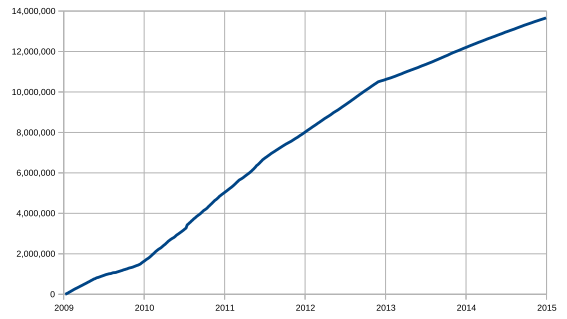
\includegraphics[height=2.5cm]{figs/bitcoin-total-evolution} \\
Bitcoins en circulación \\
\end{column}%
\hfill%
\begin{column}{.54\textwidth}
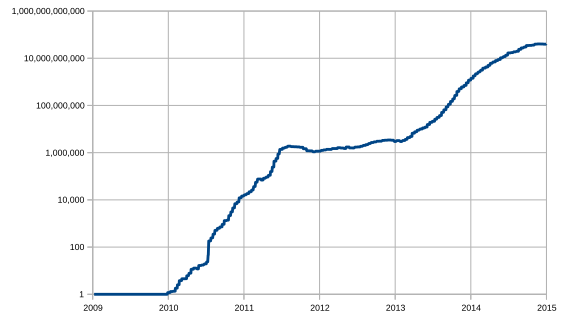
\includegraphics[height=2.5cm]{figs/bitcoin-difficulty} \\
Dificultad de producción de bloque (log) \\
\end{column}%
\end{columns}
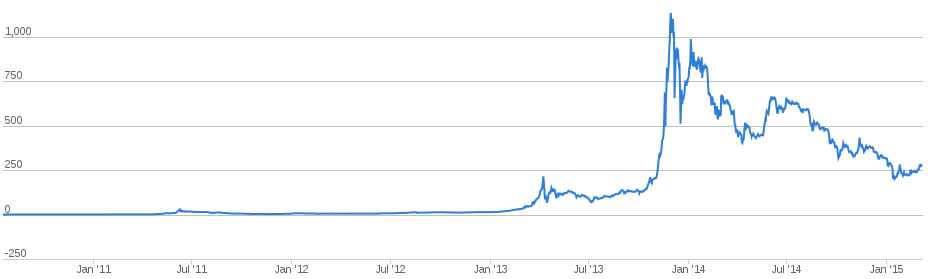
\includegraphics[width=11cm]{figs/bitcoin-usd-evolution} \\
BTC / USD \\
\end{center}
\begin{flushright}
\url{https://bitcoinaverage.com/charts}
\end{flushright}

\end{frame}

%%-----------------------------------------------------
\begin{frame}
\frametitle{La cadena de bloques}

{\large
\begin{columns}[T]
\begin{column}{.56\textwidth}
\begin{itemize}
\item Las transacciones se publican, y con ellas se generan bloques
\item En cuanto un nuevo bloque es publicado, se empieza a calcular el siguiente
\item Resultado: cadena de bloques, generada con mucho trabajo (muy robusta)
\item Puede usarse como marca de tiempo e integridad de documentos (notaría)
\end{itemize}
\end{column}%
\hfill%
\begin{column}{.40\textwidth}

Cada bloque contiene:
\begin{itemize}
\item SHA-256 del anterior
\item Lista de transacciones
\item Prueba de trabajo: objetivo de dificultad y nonce (difícil de generar, fácil de comprobar)
\end{itemize}

``Gana'' el primero que publica
\end{column}%
\end{columns}
}

\begin{flushright}
\url{http://en.wikipedia.org/wiki/Bitcoin} \\
\url{http://gsyc.es/~mortuno/sro/bitcoin.pdf} \\
\end{flushright}

\end{frame}





